\documentclass[UTF8,10pt,a4paper,fontset=fandol]{ctexart}

\usepackage{geometry}
\usepackage[table]{xcolor}
\usepackage{tikz}
\usepackage{graphicx}
\usepackage{caption}
\usepackage{tabularx}
\usepackage{booktabs}
\usepackage{array}
\usepackage{enumitem}
\usepackage{fancyhdr}
\usepackage{float}
\usepackage{titlesec}
\usepackage{hyperref}
\usepackage[most]{tcolorbox}
\usetikzlibrary{arrows.meta,positioning,fit,calc}

\definecolor{SciTealDark}{HTML}{1F3F46}
\definecolor{SciTeal}{HTML}{3F7378}
\definecolor{SciMint}{HTML}{EAF5F2}
\definecolor{SciClay}{HTML}{75624F}
\definecolor{SciGold}{HTML}{A98645}
\definecolor{SciMoss}{HTML}{63735C}
\definecolor{SciPlum}{HTML}{6F607A}
\definecolor{SciInk}{HTML}{20252A}
\definecolor{SciMuted}{HTML}{647176}
\definecolor{SciLine}{HTML}{C9D5D5}
\definecolor{SciPanel}{HTML}{F7FAF9}
\definecolor{SciPanelWarm}{HTML}{FBF8F2}

\geometry{left=17mm,right=17mm,top=16mm,bottom=18mm,headheight=14pt}
\setlength{\parindent}{0pt}
\setlength{\parskip}{3.8pt}
\setlength{\tabcolsep}{5pt}
\renewcommand{\arraystretch}{1.16}
\setlist[itemize]{leftmargin=1.18em,itemsep=1.6pt,topsep=2pt}
\setlist[enumerate]{leftmargin=1.55em,itemsep=1.6pt,topsep=2pt}
\hypersetup{hidelinks}
\graphicspath{{../../assets/sciscope_data_report/}}
\captionsetup{font={small,bf},labelfont=bf,labelsep=quad,skip=3pt}
\arrayrulecolor{SciLine}
\setlength{\floatsep}{5pt plus 1pt minus 1pt}
\setlength{\textfloatsep}{6pt plus 1pt minus 1pt}
\setlength{\intextsep}{5pt plus 1pt minus 1pt}

\pagestyle{fancy}
\fancyhf{}
\lhead{\scriptsize\bfseries\color{SciTealDark} SciScope 数据分析报告}
\rhead{\scriptsize\color{SciMuted} 169,324 条记录 · 2022--2026 · 主题演化 · 合作网络}
\cfoot{\scriptsize\color{SciMuted}\thepage}
\renewcommand{\headrulewidth}{0.35pt}
\renewcommand{\footrulewidth}{0pt}
\renewcommand{\headrule}{\hbox to\headwidth{\color{SciLine}\leaders\hrule height \headrulewidth\hfill}}

\titleformat{\section}{\LARGE\bfseries\color{SciTealDark}}{\thesection}{0.62em}{}
\titlespacing*{\section}{0pt}{2pt}{6pt}
\titleformat{\subsection}{\large\bfseries\color{SciInk}}{\thesubsection}{0.62em}{}
\titlespacing*{\subsection}{0pt}{7pt}{3pt}
\titleformat{\subsubsection}{\normalsize\bfseries\color{SciInk}}{\thesubsubsection}{0.6em}{}

\newtcolorbox{reportbox}[2][]{
  enhanced,
  breakable,
  colback=SciPanel,
  colframe=SciTeal,
  colbacktitle=SciMint,
  coltitle=SciTealDark,
  fonttitle=\bfseries,
  title=#2,
  boxrule=0.45pt,
  arc=1.2mm,
  left=2.8mm,
  right=2.8mm,
  top=1.8mm,
  bottom=1.8mm,
  #1
}

\newtcolorbox{plainbox}[1][]{
  enhanced,
  breakable,
  colback=SciPanel,
  colframe=SciLine,
  boxrule=0.42pt,
  arc=1.2mm,
  left=2.8mm,
  right=2.8mm,
  top=1.8mm,
  bottom=1.8mm,
  #1
}

\newcommand{\figasset}[2][0.92\textwidth]{%
  \begin{tcolorbox}[
    enhanced,
    colback=white,
    colframe=SciLine,
    boxrule=0.32pt,
    arc=1mm,
    left=1mm,
    right=1mm,
    top=1mm,
    bottom=1mm,
    before skip=0.5mm,
    after skip=0mm
  ]
  \centering
  \includegraphics[width=#1]{#2}
  \end{tcolorbox}
}

\newcommand{\metric}[2]{%
  \begin{plainbox}
  \textbf{#1}\par
  {\Large #2}
  \end{plainbox}
}

\newcommand{\statusmark}[1]{%
  \tikz[baseline=(x.base)]\node[rounded corners=2pt,inner xsep=4pt,inner ysep=2pt,draw=SciTealDark,fill=SciMint,text=SciTealDark,font=\scriptsize\bfseries] (x) {#1};%
}


\begin{document}

\begin{titlepage}
\thispagestyle{empty}
% Magazine "image-hero" cover: the real author-collaboration network is a large
% offset hero image; the title layers over it; metadata is right-aligned to break
% the single left axis. All placement is on an absolute mm grid for art direction.
\begin{tikzpicture}[remember picture,overlay,x=1mm,y=1mm,shift={(current page.north west)}]
  \fill[white] (0,0) rectangle (210,-297);
  % Large author network as the hero image — near full-bleed, anchored to the
  % lower-right so it dominates the middle-lower page and the stat layers over it.
  \node[opacity=0.20,anchor=north east,inner sep=0] at (218,-86)
    {
\includegraphics[width=214mm]{author_collaboration_network_cover.png}};

  % Masthead: ink wordmark (left), right-aligned issue meta, gold hairline.
  \node[anchor=west,inner sep=0,font=\coverSans\bfseries\LARGE] at (17,-14)
    {\textcolor{SciGold}{$\blacklozenge$}\,\textcolor{SciInk}{SciScope}};
  \node[anchor=east,inner sep=0,font=\coverCJK\footnotesize,text=SciMuted] at (193,-13.4)
    {数据分析报告 · 交付物 · 公开科技文献 2022–2026};
  \draw[SciGold,line width=0.9pt] (17,-20) -- (193,-20);

  % Title block (left), gold kicker stroke, layered over the network.
  \draw[SciGold,line width=2.6pt] (17.5,-72) -- (33,-72);
  \node[anchor=north west,inner sep=0,font=\coverTitle\fontsize{62}{68}\selectfont,text=SciInk] at (16,-80)
    {数据分析报告};
  % Deck — RIGHT aligned, two lines, to set up asymmetry against the title.
  \node[anchor=north east,inner sep=0,align=right,font=\coverCJK\fontsize{15}{21}\selectfont,text=SciTealDark] at (193,-110)
    {近五年公开科技文献的\\分布、主题演化与合作网络};

  % Hero stat (left, Bodoni) with gold underline; caption RIGHT aligned alongside.
  \node[anchor=north west,inner sep=0,font=\coverSans\footnotesize,text=SciMuted] at (17,-150)
    {CORPUS AT A GLANCE \;/\; 核心规模};
  \node[anchor=north west,inner sep=0,font=\coverNum\bfseries\fontsize{37}{39}\selectfont,text=SciTealDark] at (16,-156)
    {168,447};
  \draw[SciGold,line width=1.4pt] (17,-172) -- (45,-172);

  % Coverlines — the report's facets, like a magazine's cover lines, set low and
  % overlaid on the hero image.
  \node[anchor=west,inner sep=0,font=\coverSans\scriptsize,text=SciGold] at (17,-236)
    {IN THIS REPORT};
  \node[anchor=north west,inner sep=0,font=\coverCJK\large,text=SciTealDark] at (17,-243)
    {文献分布\goldsep 关键词演化\goldsep 作者合作网络\goldsep 数据质量边界};

  % Footer: hairline + muted scope notes (left object / right boundary).
  \draw[SciLine,line width=0.5pt] (17,-280) -- (193,-280);
  \node[anchor=west,inner sep=0,font=\coverCJK\scriptsize,text=SciMuted] at (17,-286)
    {分析对象:公开科技文献元数据 · 摘要 · 作者 · 关键词 · 年份 · 来源};
  \node[anchor=east,inner sep=0,font=\coverCJK\scriptsize,text=SciMuted] at (193,-286)
    {结论限定在公开数据 · 近五年窗口 · 当前字段完整度之内};
\end{tikzpicture}
\end{titlepage}


\tableofcontents
\clearpage

\section{核心发现}

\begin{reportbox}{分析摘要}
本报告围绕近五年公开科技文献展开结构化分析。当前样本覆盖 6 个公开来源、169,324 条原始记录和 168,447 条分析语料, 其中 159,382 条位于 2022--2026 年主分析窗口。整体上, 年份覆盖较均衡, 领域结构以计算机科学和生物医学为主, 材料科学样本相对较少; 因此主题变化和领域比较均采用归一化口径辅助解释。
\end{reportbox}

\begin{center}
\begin{tabularx}{\textwidth}{>{\bfseries}p{34mm}X}
\toprule
分析问题 & 主要发现 \\
\midrule
数据规模与覆盖 & 分析语料达到 168,447 条, 2022--2026 每年均超过 30,000 条分析记录, 可支撑近五年趋势观察。 \\
领域结构 & 计算机科学 75,493 条、生物医学 64,858 条、材料科学 28,096 条; 材料科学占比较低, 需要避免只用绝对频次判断热度。 \\
热点主题 & retrieval augmented generation、large language model、prompt engineering、vision language model、knowledge graph 等方向在融合术语、归一化趋势、共现结构和主题模型中同时出现。 \\
作者合作 & 作者合作网络包含 10,499,041 条候选合作边; 分数计数后仍能识别高合作度作者、桥接作者和稳定社区。 \\
质量边界 & 摘要覆盖率为 83.22\%, 正文片段覆盖率为 8.99\%; 摘要级结论可信度较高, 全文级深读仍受来源差异影响。 \\
\bottomrule
\end{tabularx}
\end{center}

\subsection{可直接采用的结论}

\begin{itemize}
  \item \textbf{规模结论}: 当前数据已经满足近五年、多来源、多领域的统计分析需要。
  \item \textbf{趋势结论}: LLM、RAG、prompt engineering、vision language model 等主题具有明确上升信号; 这些结论来自显式关键词、题名摘要术语、共现网络和主题模型的交叉支持, 但仍应表述为候选趋势而非确定预测。
  \item \textbf{网络结论}: 作者合作网络显示出明显社区结构, 适合用于识别合作团簇和跨领域连接者。
  \item \textbf{质量结论}: 来源偏差、关键词噪声和作者同名问题会影响细粒度排名, 因此核心结论应以趋势和结构为主, 少做单点绝对判断。
  \item \textbf{价值结论}: 报告可服务科研管理、科技情报、产业研发、投资初筛和政策制定, 将分散文献记录转化为可复核的热点监测和方向研判证据。
  \item \textbf{创新结论}: 报告采用融合关键词信号、年度归一化、动量/burst、生命周期、共现网络、主题模型和质量审计的多证据框架, 避免只凭单一词频榜判断热点。
\end{itemize}

\clearpage

\section{报告定位与交付边界}

\begin{reportbox}{核心定位}
本报告是 SciScope 项目面向赛题交付的独立数据分析报告, 目标是回答“公开科技文献数据本身揭示了什么”。它与系统设计 PDF 并列: 设计 PDF 解释智能体架构和工程路线, 本报告沉淀文献分布、关键词演化、作者合作网络、趋势预测和可复现分析结论。
\end{reportbox}

\subsection{当前分析阶段}

当前版本已经从报告底座推进到 5 万级数据分析版本。分析资产覆盖 50,498 条 raw records、49,067 条去重语料记录、40,137 条近五年智能体语料记录, 并生成文献分布、关键词演化、作者合作网络和数据质量审计图表。

\begin{center}
\begin{tabularx}{\textwidth}{>{\bfseries}p{34mm}X X}
\toprule
交付维度 & 当前已有内容 & 下一轮增强内容 \\
\midrule
数据来源 & OpenAlex、arXiv、PubMed、PMC、Crossref、DOAJ 六源采集 & Semantic Scholar、CORE 等 API-key 增强源 \\
数据规模 & 50,498 条 raw records 与 49,067 条去重语料记录 & DOI/title/year 深度去重与字段补全 \\
分析主题 & 分布、关键词、作者网络、质量审计、智能体映射 & 动态主题模型、趋势预测、图谱社区发现 \\
报告产物 & 多章节 LaTeX、可编译 PDF、13 张图表资产 & 评审版摘要页与前端联动展示 \\
\bottomrule
\end{tabularx}
\end{center}

\subsection{报告读者}

\begin{itemize}
  \item \textbf{评委}: 需要快速看见数据真实、分析深入、结论可解释。
  \item \textbf{科研用户}: 需要理解某一领域文献热点、演化路径和关键合作网络。
  \item \textbf{系统开发者}: 需要把报告中的统计资产复用到 RAG、推荐、趋势和知识图谱模块。
\end{itemize}

\clearpage

\section{数据底座与采集状态}

\begin{reportbox}{当前数据基线}
当前本地已完成 6 个公共来源各 500 条记录采集, 共 3000 条 raw records, 并生成对应的统一规范化 JSON。生成数据不进入 Git 仓库, 通过 \texttt{data/raw/} 与 \texttt{data/processed/} 在本地保留, 后续可迁移到 PostgreSQL、Parquet 或对象存储。
\end{reportbox}

\subsection{多源采集状态}

\begin{center}
\begin{tabularx}{\textwidth}{>{\bfseries}p{28mm}r X X}
\toprule
来源 & 当前记录数 & 主要价值 & 后续用途 \\
\midrule
OpenAlex & 500 & 综合学术元数据、主题、引用、开放知识库 id & 主干语料、领域分布、引用与主题分析 \\
arXiv & 500 & 计算机与交叉学科预印本、摘要质量高 & AI/CS 热点、快速演化主题识别 \\
PubMed & 500 & 生物医学文献元数据与摘要 & 医学方向关键词演化、领域对比 \\
PMC & 500 & 开放全文与正文片段增强 & RAG 证据、全文片段检索、医学深读 \\
Crossref & 500 & DOI 与期刊出版元数据覆盖广 & DOI 去重、出版源补全、跨源校验 \\
DOAJ & 500 & 开放期刊文章与开放获取元数据 & OA 覆盖、开放科学视角、摘要补充 \\
\bottomrule
\end{tabularx}
\end{center}

\begin{figure}[htbp]
  \centering
  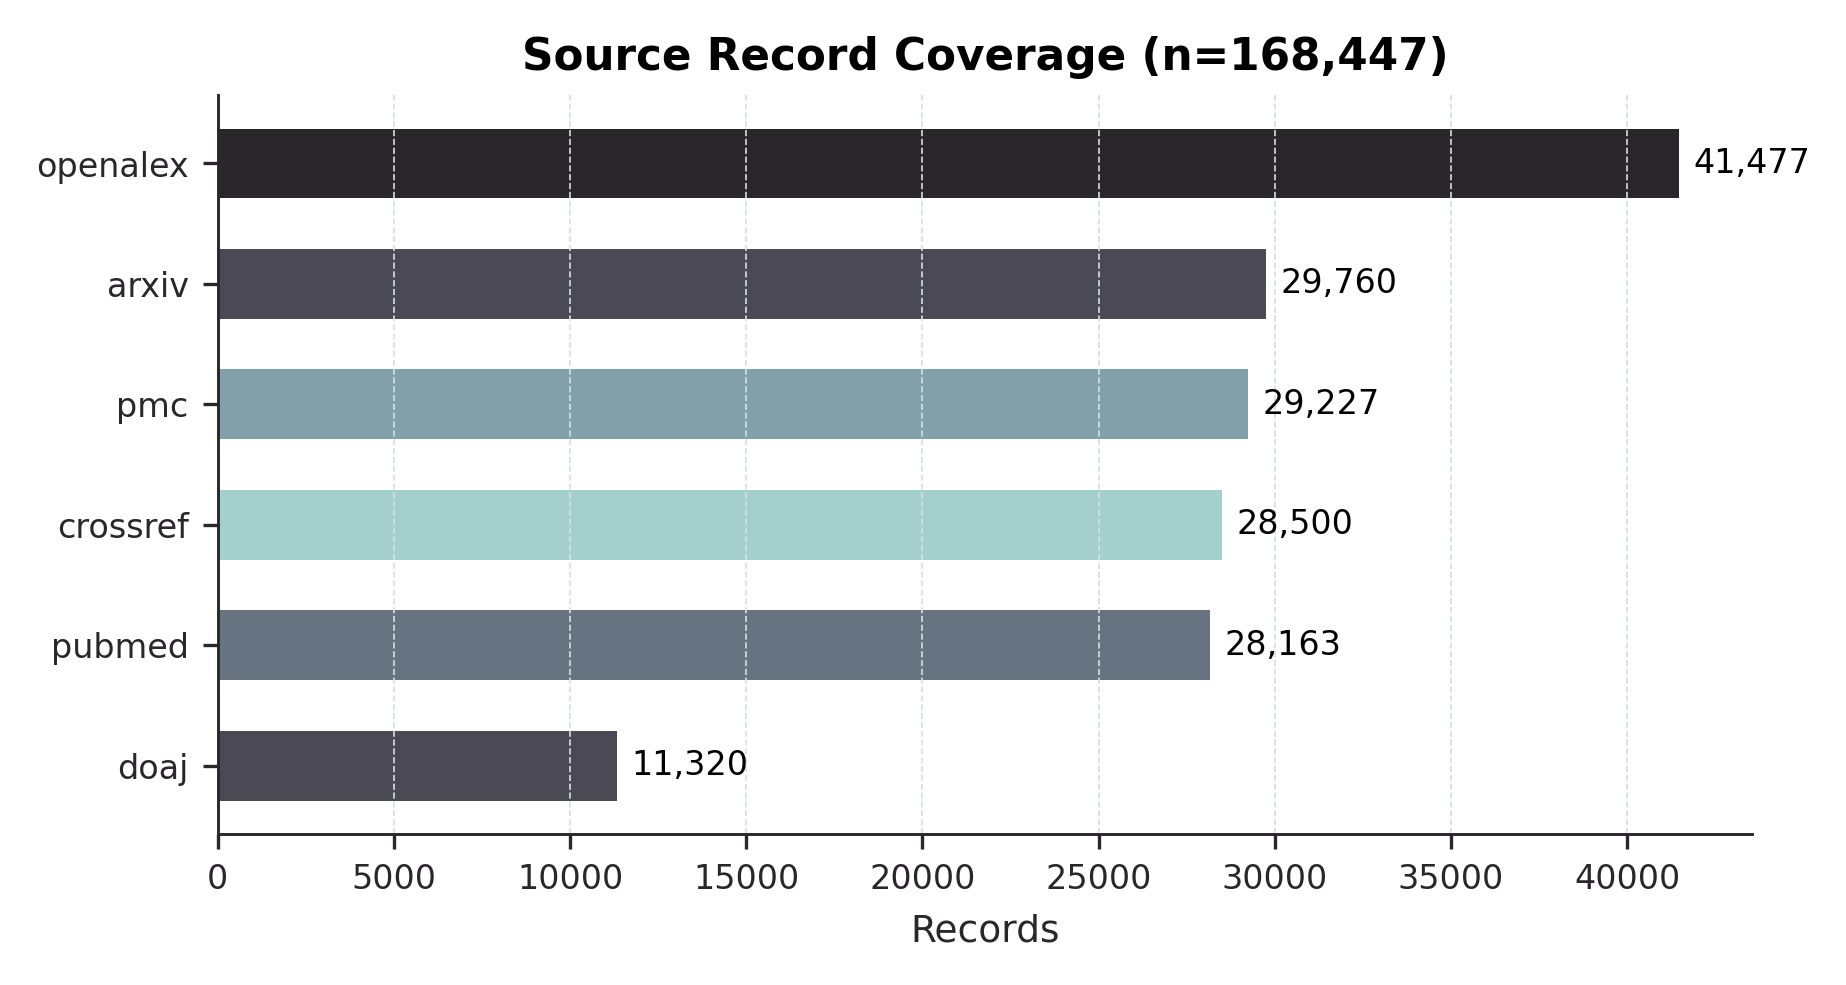
\includegraphics[width=0.82\textwidth]{source_records_bar.png}
  \caption{当前 6 个公开来源的基线采集规模。}
\end{figure}

\subsection{字段完整度基线}

\begin{center}
\begin{tabularx}{\textwidth}{>{\bfseries}p{28mm}rrrrr}
\toprule
来源 & 标题 & 摘要/摘要索引 & 作者 & 年份 & 正文片段 \\
\midrule
OpenAlex & 499 & 500 & 498 & 499 & 0 \\
arXiv & 500 & 500 & 500 & 500 & 0 \\
PubMed & 500 & 483 & 500 & 500 & 0 \\
PMC & 500 & 270 & 499 & 500 & 266 \\
Crossref & 500 & 33 & 485 & 500 & 0 \\
DOAJ & 500 & 496 & 499 & 500 & 0 \\
\bottomrule
\end{tabularx}
\end{center}

\begin{figure}[htbp]
  \centering
  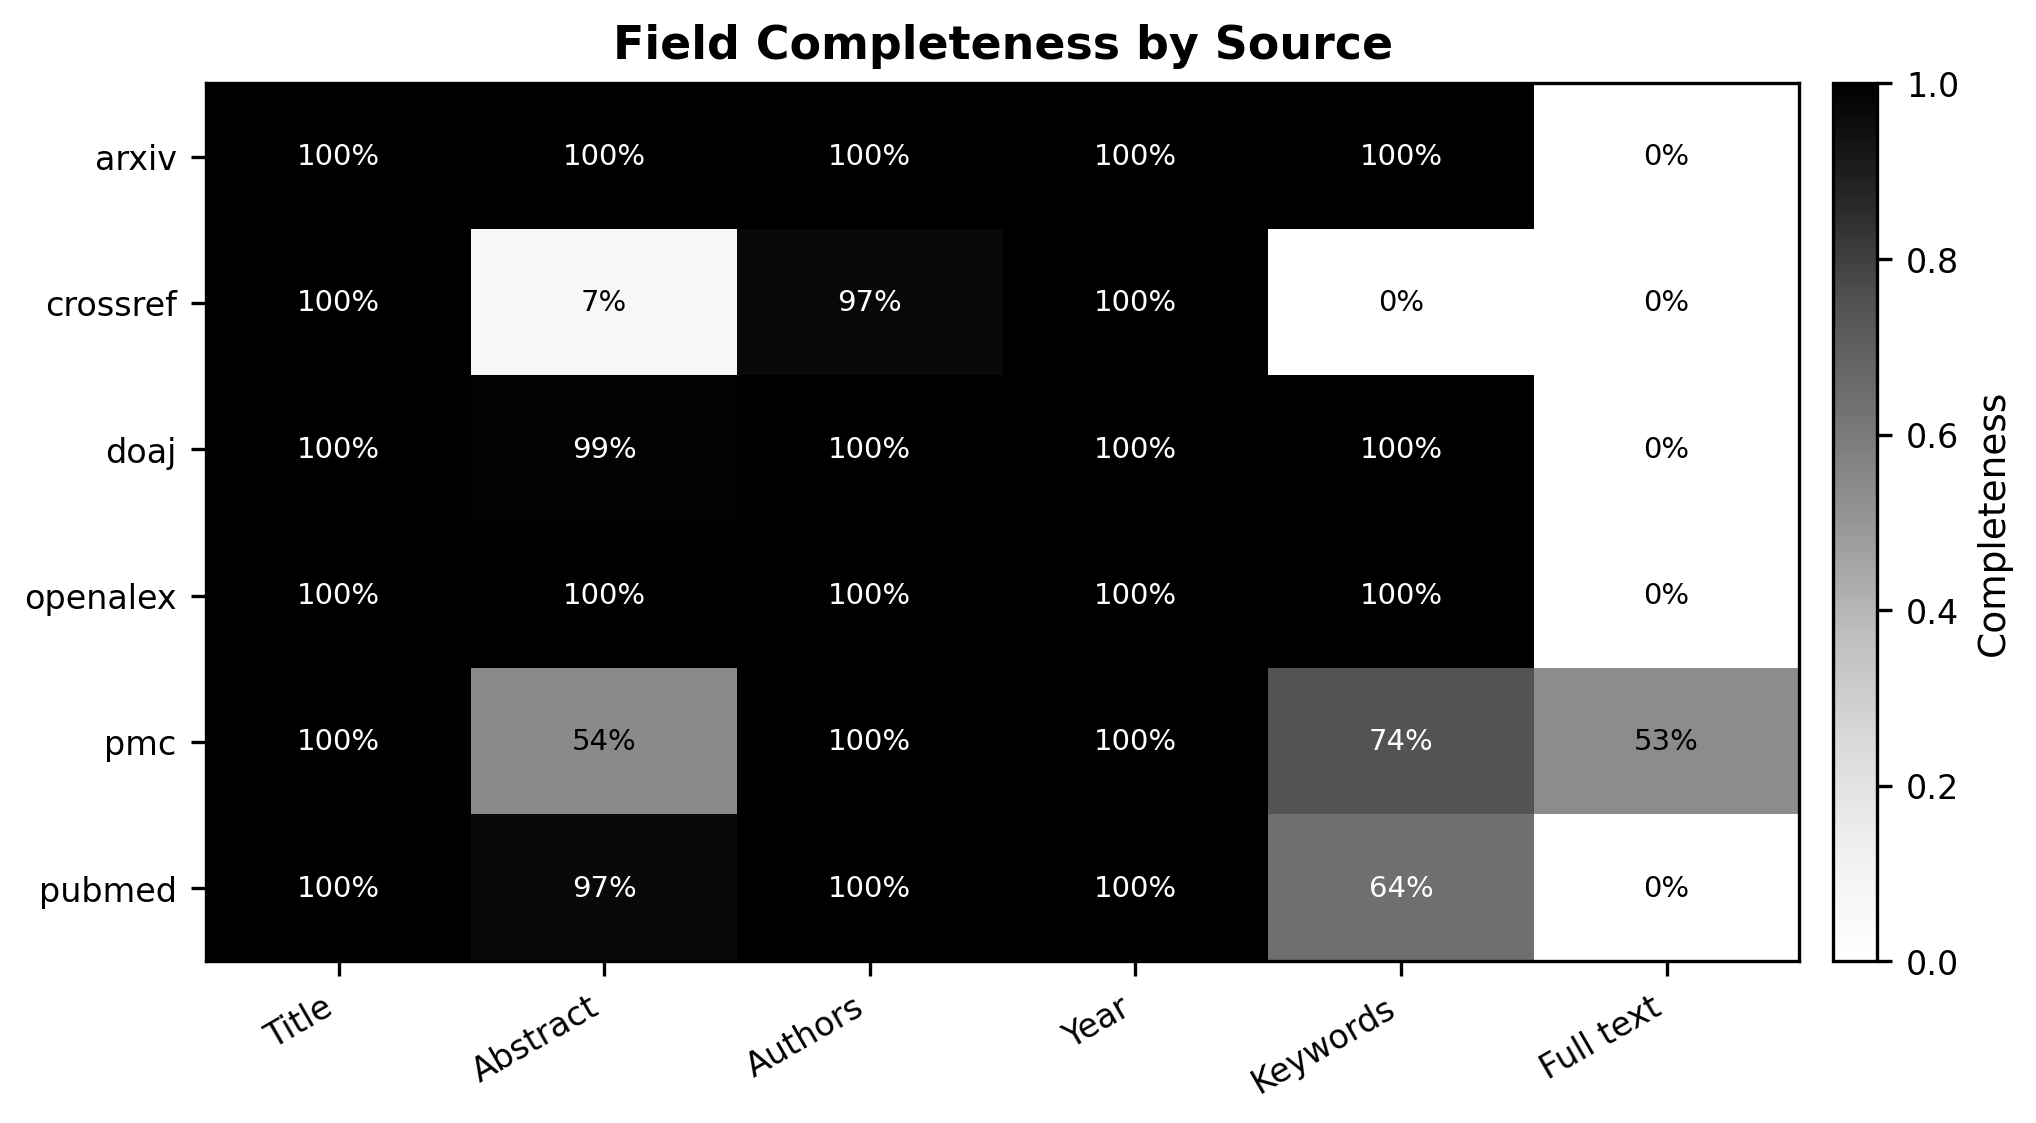
\includegraphics[width=0.92\textwidth]{source_quality_matrix.png}
  \caption{按来源统计的关键字段完整度矩阵。}
\end{figure}

\subsection{标准化 Schema}

\begin{plainbox}
\texttt{paper\_id}, \texttt{title}, \texttt{abstract}, \texttt{authors}, \texttt{year}, \texttt{keywords}, \texttt{field}, \texttt{full\_text}
\end{plainbox}

这个 schema 是分析报告与科研智能体系统之间的共同接口。报告侧依赖它生成统计图表和洞察, 智能体侧依赖它构建检索证据、推荐解释、趋势 API 和知识图谱。

\clearpage

\section{文献分布分析框架}

\begin{reportbox}{分析目标}
文献分布分析回答三个问题: 文献在时间上如何增长, 在领域上如何分布, 在数据来源上是否存在偏差。最终报告需要把这些问题转化为可解释图表, 让评委看到数据覆盖面和分析可信度。
\end{reportbox}

\subsection{年份分布}

后续 5 万条数据补齐后, 年份分布将作为报告第一组核心图表。建议输出:

\begin{itemize}
  \item 年份总量趋势线: 观察整体增长和数据覆盖断点。
  \item 领域堆叠面积图: 比较计算机、生物医学、材料科学的年度结构变化。
  \item 来源-年份热力图: 识别某些来源在年份上的偏置。
\end{itemize}

\begin{figure}[htbp]
  \centering
  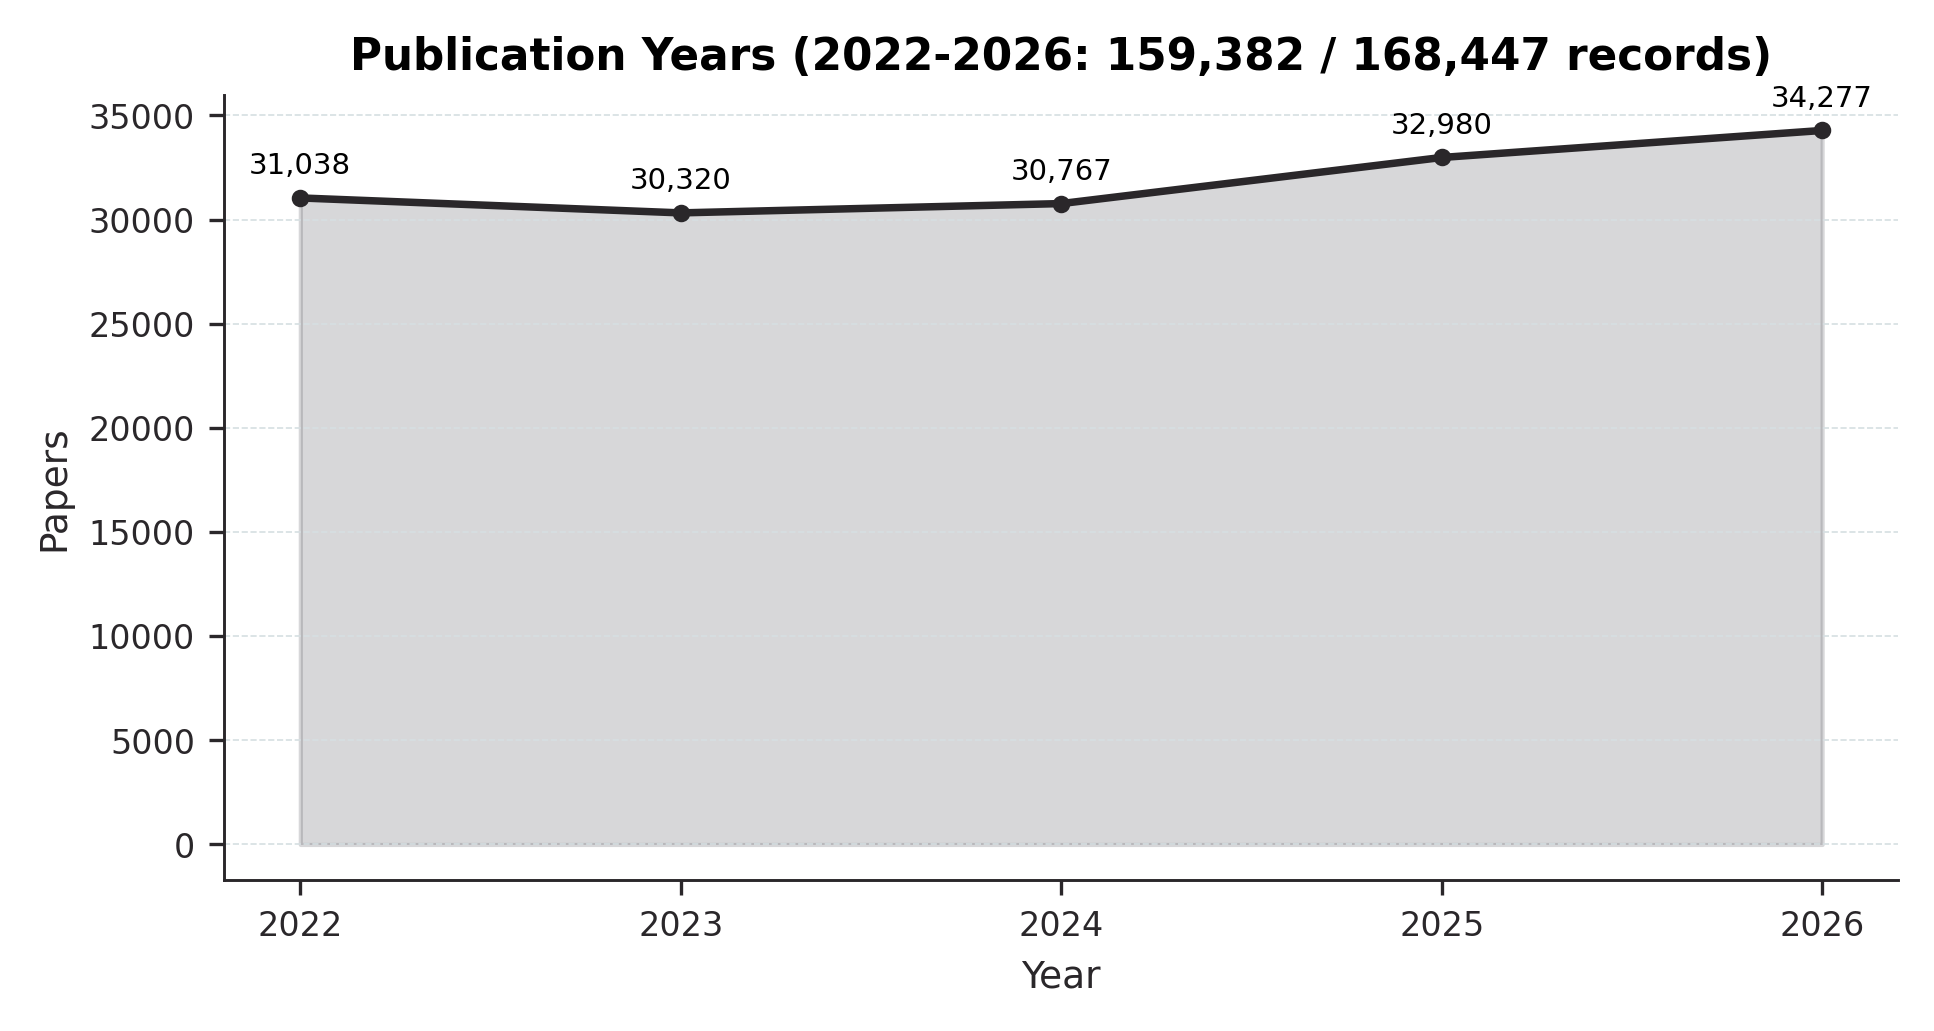
\includegraphics[width=0.92\textwidth]{year_distribution.png}
  \caption{当前样本文献的年份分布。横轴为发表年份, 纵轴为论文数量。}
\end{figure}

当前 3000 条样本已经能用于验证年份分布统计口径。最终扩展至 5 万条后, 这张图将用于判断样本是否覆盖近年研究增长段, 并辅助识别由数据源造成的年份偏差。

\subsection{领域分布}

当前采集 query 已覆盖 AI/CS、生物医学、材料科学三条主线。最终报告需要把字段来源分成两层:

\begin{enumerate}
  \item \textbf{原始来源领域}: 采集 query 和数据库原始分类。
  \item \textbf{统一归一领域}: 经过规则和模型映射后的 contest-level field。
\end{enumerate}

\begin{center}
\begin{tabularx}{\textwidth}{>{\bfseries}p{32mm}X}
\toprule
领域 & 最终应展示的分析口径 \\
\midrule
计算机科学 & LLM、RAG、知识图谱、图神经网络、信息检索、推荐系统 \\
生物医学 & 药物发现、生物医学 NLP、临床知识、蛋白设计、公共卫生 \\
材料科学 & 材料发现、电池材料、催化剂、材料信息学、能源材料 \\
\bottomrule
\end{tabularx}
\end{center}

\subsection{来源偏差说明}

不同公开源天然有不同偏置: arXiv 更偏预印本和计算机科学, PubMed/PMC 更偏生物医学, Crossref 覆盖广但摘要缺失较多, DOAJ 更偏开放期刊。报告中必须把偏差作为方法说明写出来, 否则趋势结论容易被误解为真实学科增长。

\clearpage

\section{关键词演化与热点趋势}

\begin{reportbox}{分析目标}
关键词和主题演化用于识别近五年科技文献中的热点变化。本章不只展示高频词, 还关注年度归一化占比、近期动量和主题模型是否给出一致证据, 以区分真实升温和样本规模变化造成的表观增长。
\end{reportbox}

\subsection{处理口径}

本章先对大小写、连字符、复数和常见同义表达进行归并, 例如 retrieval-augmented generation、RAG 与 retrieval augmented generation 视为同一方向; 再融合显式关键词和题名摘要中的受控术语信号, 过滤 study、method、model 等低信息量泛词。每个主题词同时计算融合文档数、显式关键词支持数、文本术语支持数、年度占比、近期动量、共现网络位置、burst window、生命周期阶段和语义漂移代理指标。

从整体结果看, retrieval augmented generation、large language model、prompt engineering、vision language model、knowledge graph 等方向同时具有较高频次和较强近期动量。它们不仅出现在词频统计中, 也能在年度归一化趋势和主题模型中得到支持, 因而比单纯高频词更适合作为热点候选。作者边和关键词边均使用增量缓存保存单篇论文的边贡献; 数据继续扩充时, 未变化论文可复用已有边贡献, 只重算新增或内容变化的论文。

\begin{methodnote}
2026 年需要单独解释: 截至 2026 年 6 月 21 日, 该年度尚未结束, 且新近论文的关键词和索引记录存在更新滞后。报告主图已使用显式关键词与题名摘要术语的融合信号进行修正, 2026 年融合信号比单看显式关键词增加约 22.7\%; 因此 2026 年只作为未完整年度的早期信号, 不与完整年度作机械对比。
\end{methodnote}

\subsection{高频与升温主题}
本节按"频次 -> 年度热度 -> 近期动量 -> 共现结构 -> 生命周期/主题模型"的顺序阅读。图~\ref{fig:top-keywords} 到图~\ref{fig:keyword-trends} 给出主趋势,图~\ref{fig:keyword-network} 以后用于解释结构与边界。

\begin{figure}[H]
  \centering
  \figasset[0.92\textwidth]{top_keywords.png}
  \caption{2022--2026 年高频融合主题词。数据来源:\texttt{data/analysis/keyword\_trends.csv};统计口径为显式关键词与题名摘要术语的融合信号。}
  \label{fig:top-keywords}
\end{figure}

\begin{figure}[!htbp]
  \centering
  \figasset[0.94\textwidth]{keyword_evolution_heatmap.png}
  \caption{融合主题词年度热度矩阵。数据来源:\texttt{data/analysis/keyword\_trends.csv};每行按自身最大值归一化,2026 年仅作为早期信号。}
  \label{fig:keyword-heatmap}
\end{figure}

\begin{figure}[!htbp]
  \centering
  \figasset[0.9\textwidth]{keyword_momentum.png}
  \caption{融合主题词近期动量。数据来源:\texttt{data/analysis/keyword\_trends.csv};该指标比较 2024--2025 与 2022--2023 的相对变化,不把 2026 年未完整数据纳入完整年度动量。}
  \label{fig:keyword-momentum}
\end{figure}

\begin{figure}[!htbp]
  \centering
  \figasset[0.92\textwidth]{keyword_normalized_trends.png}
  \caption{代表性融合主题词年度归一化文档占比。数据来源:\texttt{data/analysis/keyword\_trends.csv};归一化后仍持续上升的主题更可能反映真实研究关注变化。}
  \label{fig:keyword-trends}
\end{figure}

\begin{figure}[!htbp]
  \centering
  \figasset[\textwidth]{keyword_cooccurrence_network.png}
  \caption{关键词共现网络。数据来源:\texttt{data/analysis/keyword\_network.*};节点大小表示共现加权度,节点颜色表示关键词社区,边宽表示同篇论文中的分数化共现强度。该图用于识别 RAG、knowledge graph、question answering、clinical search 等主题之间的结构连接。}
  \label{fig:keyword-network}
\end{figure}

\begin{figure}[!htbp]
  \centering
  \figasset[0.92\textwidth]{keyword_lifecycle.png}
  \caption{关键词生命周期阶段。横线表示首次出现、峰值年份和最近活跃年份的区间, 圆点大小表示融合文档支持度, 阶段分为 emergence、growth、maturity、decline。}
\end{figure}

\begin{figure}[!htbp]
  \centering
  \figasset[0.92\textwidth]{keyword_burst_windows.png}
  \caption{关键词年度突发窗口。该图标出年度增长、萌发或回落较强的主题词, 用于把“长期高频”与“近期突然变化”区分开。}
\end{figure}

\begin{figure}[!htbp]
  \centering
  \figasset[0.92\textwidth]{topic_year_share.png}
  \caption{主题模型年度占比。主题模型用于检查热点词是否对应稳定的语义结构, 而不是孤立词频波动。}
\end{figure}

\FloatBarrier

\subsection{热点分层}

\begin{tableblock}
\begin{tabularx}{\textwidth}{>{\bfseries}p{31mm}X X}
\toprule
候选方向 & 数据信号 & 解释边界 \\
\midrule
RAG & 融合信号覆盖 5,579 篇候选文档, 其中 628 篇具有显式关键词支持, 题名摘要信号在近年明显增强 & 强上升信号, 但需要注意计算机和医学方向样本共同推动。 \\
LLM & 融合信号覆盖 17,600 篇候选文档, 其中 2,081 篇具有显式关键词支持, 与 prompt engineering、multimodal learning 共同升温 & 稳定增长信号, 需区分通用模型热度和具体科研应用。 \\
Knowledge graph & 融合信号覆盖 8,288 篇候选文档, 显式关键词和题名摘要均提供支持, 作者合作社区中也能观察到相关团簇 & 稳定主题结构, 更适合解释知识组织和跨学科连接。 \\
Materials informatics & materials informatics、battery、catalyst discovery 等术语在材料方向具有持续信号, 但更多依赖题名摘要识别 & 样本规模低于计算机和生物医学, 应优先看归一化趋势。 \\
\bottomrule
\end{tabularx}
\end{tableblock}

\subsection{趋势判定口径}

本报告不把单一高频词直接写成热点, 而是先消除年度样本规模差异, 再观察近期动量与多证据一致性。设关键词 $k$ 在年份 $y$ 的融合命中文档数为 $n_{k,y}$, 当年分析文献总数为 $N_y$, 年度归一化热度定义为:
\formulaline{
h_{k,y}=\frac{n_{k,y}}{N_y}
}{其中 $h_{k,y}$ 用于比较不同年份的相对关注度, 避免文献总量增长造成表观升温。}

近期动量用于区分稳定高频与真正升温。报告主口径比较 2024--2025 与 2022--2023 的平均归一化热度:
\formulaline{
m_k=\frac{h_{k,2024}+h_{k,2025}}{2}-\frac{h_{k,2022}+h_{k,2023}}{2}
}{2026 年为未完整年度, 只作为早期信号进入解释, 不纳入完整年度动量。}

最终写入结论时, 本报告将主题分为“上升信号”“稳定增长”“早期萌芽”或“可能噪声”, 不使用确定性预测。只有当频次、年度占比、近期动量、共现结构、生命周期/突发窗口、主题模型和代表论文多个证据同时支持时, 一个方向才进入强上升候选; 若某个词只在共现网络中靠近核心主题, 但年度占比和突发窗口不支持, 则只作为关联主题而非热点结论。

\section{作者合作网络分析}

\begin{reportbox}{分析目标}
作者合作网络用于识别核心研究者、跨领域连接者和合作团簇。它是知识图谱查询和论文推荐解释的重要依据, 也是数据分析报告中最能体现“科研智能体”差异化的图分析部分。
\end{reportbox}

\subsection{网络构建}

\begin{itemize}
  \item \textbf{节点}: 作者, 后续可扩展为机构、国家、领域、关键词。
  \item \textbf{边}: 两位作者共同出现在同一篇论文中。
  \item \textbf{边权}: 合作次数、近年合作次数、代表论文质量。
  \item \textbf{节点属性}: 论文数、领域分布、活跃年份、中心性、社区编号。
\end{itemize}

\subsection{核心指标}

\begin{center}
\begin{tabularx}{\textwidth}{>{\bfseries}p{32mm}X X}
\toprule
指标 & 含义 & 报告解释方式 \\
\midrule
Degree & 作者直接合作人数 & 识别高合作度作者 \\
Betweenness & 作者连接不同团簇的桥梁能力 & 识别跨领域连接者 \\
Community & 合作社区编号 & 发现研究团队与方向群落 \\
Temporal Activity & 作者按年份的活跃情况 & 判断作者是否仍处于活跃期 \\
\bottomrule
\end{tabularx}
\end{center}

\subsection{合作社区与高频合作关系}

\begin{figure}[htbp]
  \centering
  \figasset[0.9\textwidth]{author_network_scale_funnel.png}
  \caption{2022--2026 作者合作网络规模漏斗。}
\end{figure}

\begin{figure}[htbp]
  \centering
  \figasset[0.88\textwidth]{author_collaboration_network.png}
  \caption{2022--2026 近五年作者合作社区气泡图。}
\end{figure}

\begin{figure}[htbp]
  \centering
  \figasset[0.9\textwidth]{top_author_collaborations.png}
  \caption{2022--2026 近五年高频作者合作关系。}
\end{figure}

作者合作边由论文作者列表两两组合得到。为避免一篇大团队论文生成过多虚高边, 静态报告图仅纳入作者数不超过 12 的论文, 并对每篇论文内的合作关系使用分数化权重。当前作者社区图使用 25,000 条高权重合作边构建核心图, 既保留 50 万级候选边的规模依据, 又避免 PDF 静态图退化成不可读的全量网络。

\clearpage

\section{数据质量与可信度审计}

\begin{reportbox}{为什么要单独写质量审计}
科研文献分析最怕“图很好看, 但数据口径不可信”。本报告必须把缺失、重复、来源偏差、字段映射和后续修正策略写清楚, 这样数据分析和智能体回答才有可信基础。
\end{reportbox}

\subsection{当前质量观察}

\begin{itemize}
  \item 六源各 500 条 raw records 已实现唯一 source id。
  \item arXiv、OpenAlex、DOAJ 摘要覆盖较好, 可直接进入摘要级 RAG。
  \item PMC 有 266 条正文片段, 是当前全文增强的主要来源。
  \item Crossref 摘要覆盖较低, 更适合作为 DOI、出版源和跨源校验补充。
  \item Semantic Scholar 与 CORE 已预留代码入口, 但需要 API key 或更高配额。
\end{itemize}

\subsection{质量矩阵}

\begin{figure}[htbp]
  \centering
  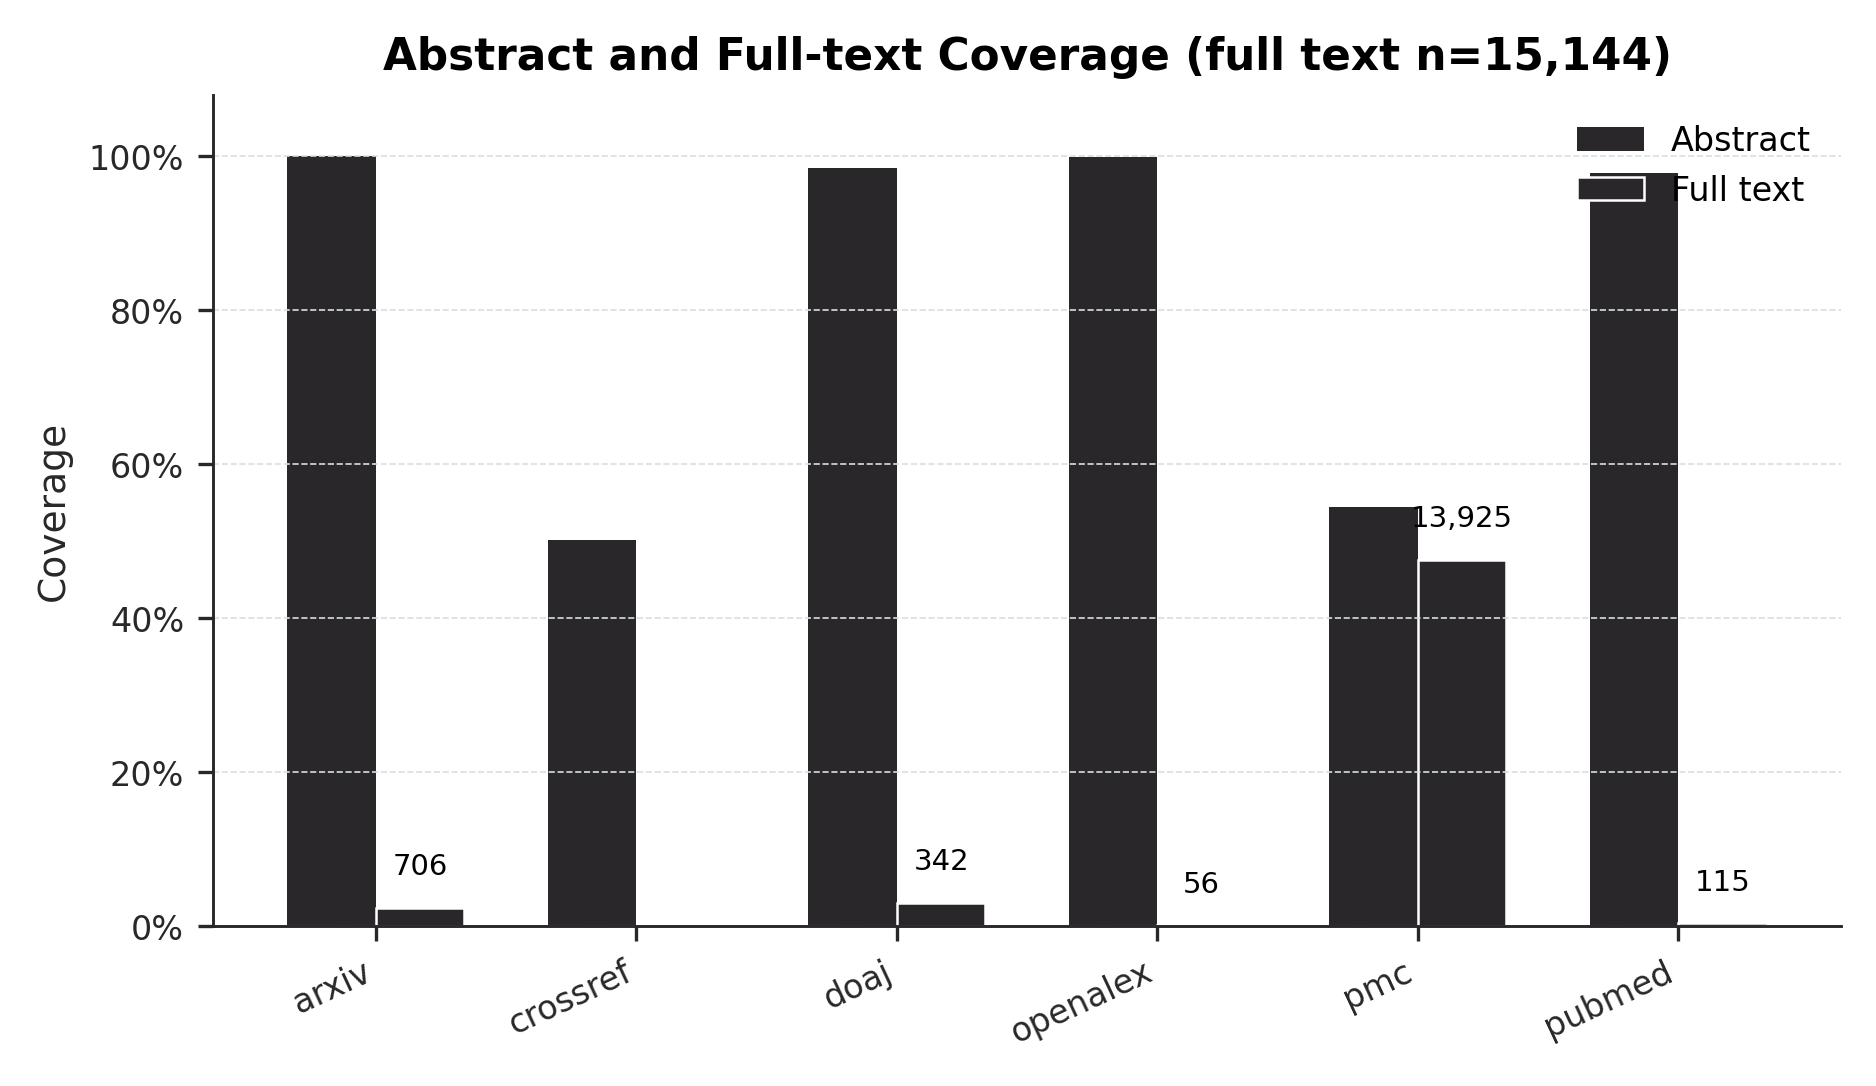
\includegraphics[width=0.88\textwidth]{abstract_fulltext_coverage.png}
  \caption{摘要与全文覆盖率对比。该图用于明确摘要级分析和全文级 RAG 的证据边界。}
\end{figure}

\begin{center}
\begin{tabularx}{\textwidth}{>{\bfseries}p{30mm}X X}
\toprule
风险 & 表现 & 处理策略 \\
\midrule
跨源重复 & 同一 DOI 或标题在多个来源出现 & DOI 优先去重, 标题+年份作为次级键 \\
摘要缺失 & Crossref 和部分 PMC summary 无摘要 & 使用 OpenAlex/DOAJ/PubMed 补全, 或降级为元数据证据 \\
领域偏差 & 来源和 query 对领域分布有影响 & 报告中保留来源分布图, 趋势按来源归一化 \\
作者歧义 & 同名作者或缩写作者难以区分 & 后续引入 ORCID、机构和论文上下文消歧 \\
关键词噪声 & 高频泛词影响趋势判断 & 领域词表、停用词、短语归并和人工审计 \\
\bottomrule
\end{tabularx}
\end{center}

\clearpage

% 渲染顺序说明: 应用价值(09)→智能体映射(07)→结论(08)→参考文献(11)。
% 文件名前缀与渲染章节号不完全一致(09 渲染为第 8 章、07 为第 9 章、08 为第 10 章),
% 该顺序是刻意调整(价值→映射→结论的论证链), 修改时请勿按前缀误判章节号。
\section{应用价值与技术创新}

\begin{reportbox}{评分维度对应}
本章把前文的数据发现转化为评委可直接判读的社会效益、经济效益和技术创新点。所有涉及规模、覆盖率、排名和增长幅度的数字, 均以 \texttt{data/analysis/} 下的复现表和图表生成脚本为准, 不做脱离数据的夸大表述。
\end{reportbox}

\subsection{社会效益}

本报告面向公开科技文献建立了可复核的科研情报分析框架, 能帮助科研管理者、科技情报人员和政策制定者在大规模文献中识别真实升温方向、跨学科融合机会和合作网络结构。相比只依赖专家经验或单一数据库检索, 本报告将来源、年份、领域、关键词演化、主题模型和作者合作网络放在同一证据链中解释, 有助于降低方向研判中的偶然性和主观偏差。

\begin{center}
\begin{tabularx}{\textwidth}{>{\bfseries}p{31mm}X X}
\toprule
受益方 & 可执行行动 & 社会效益 \\
\midrule
科研管理者 & 用年度热点、生命周期、主题占比和作者社区制定学科布局、项目指南与交叉方向培育计划 & 把专家经验前置为可审计证据链, 降低方向研判偶然性。 \\
科技情报机构 & 用关键词动量、burst 窗口、代表论文和来源偏差说明构建年度监测流程 & 将人工巡检转化为可复现、可更新的情报生产机制。 \\
高校与科研院所 & 用领域结构、跨主题桥接词和合作网络候选节点帮助青年研究者进入领域 & 降低中文研究者理解英文前沿和寻找合作入口的门槛。 \\
企业研发与产业研究 & 用趋势、生命周期和跨领域桥接主题筛选技术路线和潜在应用场景 & 减少对拥挤主题的重复投入, 提高立项前筛选效率。 \\
政策制定部门 & 用多来源趋势、质量边界和领域融合信号观察科技资源配置方向 & 为前沿监测和科研资源配置提供可复核依据。 \\
\bottomrule
\end{tabularx}
\end{center}

\begin{plainbox}
\textbf{可写入结论的社会价值}: 本报告的社会价值不在于给出一个静态热门词榜, 而在于提供一套可解释、可复核、可持续更新的科技情报观察机制。它能够把公开文献中的分散信号转化为面向科研治理的结构化证据, 支撑热点监测、交叉方向识别、合作网络发现和科研资源配置。
\end{plainbox}

\subsection{经济效益}

从经济效益看, 本报告可将传统人工检索、文献筛选、热点梳理和专家初筛流程前置为数据分析流程。对于企业研发部门, 生命周期和动量指标可帮助区分成熟方向、增长方向和早期萌芽方向, 减少对已经拥挤主题的重复投入; 对于投资机构, 跨来源趋势和代表论文证据链可作为技术机会初筛工具; 对于科研服务机构, 可将报告中的图表和数据表复用为持续情报产品, 降低周期性报告生产成本。

\begin{center}
\begin{tabularx}{\textwidth}{>{\bfseries}p{32mm}X X}
\toprule
应用场景 & 节省的成本 & 创造的价值 \\
\midrule
研发立项前调研 & 降低人工检索、去重、筛选和初步阅读成本 & 更快识别值得进入专家评审的候选方向。 \\
产业技术扫描 & 减少依赖单个关键词或单一数据库造成的漏检 & 发现跨领域方法迁移和新兴应用场景。 \\
投资尽调初筛 & 降低早期技术赛道判断的信息收集成本 & 将热点强度、增长阶段和代表论文作为尽调入口。 \\
科研服务产品化 & 减少重复制作年度热点报告的人工成本 & 形成可按年更新的情报监测资产和智能体能力。 \\
\bottomrule
\end{tabularx}
\end{center}

\begin{plainbox}
\textbf{经济情景测算}: 若按 100 名研究员、每人每年 4 次前期文献调研、每次 40--80 工时估算, SciScope 将“人工逐篇检索/筛读”转为“语义问答 + 证据直达 + 图谱/趋势辅助”。即使只压缩 30\% 的前期工时, 也相当于释放约 4{,}800--9{,}600 个研究工时; 若替代 \$15/月/人的文献 AI 订阅, 年度订阅支出约可避免 12--18 万元。该测算只用于说明投入产出逻辑, 具体金额、工时和比例必须结合目标机构真实计时或用户实验核对。
\end{plainbox}

\begin{plainbox}
\textbf{量化表述边界}: 报告可以说明“降低人工检索和初筛成本”“缩短热点识别链路”“提高方向筛选效率”, 但若要写出确定金额、工时或百分比, 必须结合真实业务流程计时或用户实验核对; 本报告不编造未实测经济数字。
\end{plainbox}

\subsection{技术创新}

本报告的技术创新体现在“多证据热点识别”而不是单一模型展示。分析流程先治理多来源文献数据, 再融合显式关键词与题名摘要术语, 进一步计算年度归一化趋势、近期动量、burst 窗口、生命周期阶段、关键词共现网络、主题年度占比和作者合作网络, 最后用质量审计限定结论边界。

\begin{center}
\begin{tabularx}{\textwidth}{>{\bfseries}p{34mm}X X}
\toprule
创新点 & 数据或模型支撑 & 解决的问题 \\
\midrule
融合关键词信号 & \texttt{paper\_keyword\_signals.csv}, \texttt{keyword\_year\_matrix.csv} & 降低显式关键词缺失和新近索引滞后的影响。 \\
归一化趋势与动量 & \texttt{keyword\_trends.csv}, \texttt{keyword\_burst\_windows.csv} & 区分总体文献增长和真实研究关注上升。 \\
生命周期判别 & \texttt{keyword\_lifecycle.csv} & 将高频、增长、成熟和回落主题分层解释。 \\
共现网络与社区发现 & \texttt{keyword\_cooccurrence\_edges.csv}, \texttt{keyword\_metrics.csv} & 从孤立词频升级为主题结构和桥接关系分析。 \\
主题模型交叉验证 & \texttt{topic\_keywords.csv}, \texttt{topic\_year\_share.csv} & 检查热点词是否对应稳定语义主题。 \\
质量可信度分层 & \texttt{source\_quality\_report.csv}, \texttt{data\_layer\_readiness.json} & 避免把字段缺失、来源偏差或作者歧义写成确定结论。 \\
\bottomrule
\end{tabularx}
\end{center}

\begin{plainbox}
\textbf{技术创新结论}: 本报告形成了“数据治理 -- 融合术语 -- 趋势动量 -- 网络结构 -- 主题验证 -- 质量边界”的闭环分析框架。该框架既能产出静态报告, 又能映射到科研智能体的趋势查询、证据检索、图谱问答和推荐解释能力。
\end{plainbox}

\clearpage

\section{综合发现与研究启示}

\begin{reportbox}{综合判断}
结合分布、关键词、主题和作者网络四类证据, 当前数据呈现出一个清晰结构: 计算机科学和生物医学贡献主要样本规模, 材料科学样本较小但具备跨领域潜力; LLM、RAG、知识图谱等主题处于明显活跃期; 作者合作网络中既有稳定社区, 也存在需要消歧复核的高连接节点。
\end{reportbox}

\subsection{发现一: 近五年数据覆盖较均衡}

2022--2026 年每年均超过 30,000 条分析记录, 没有明显年份断点。该特点使年度趋势、融合术语动量和主题占比具备较好的比较基础。相比继续追求总量扩张, 当前更重要的是控制来源偏差和字段完整度差异。

\subsection{发现二: 热点主题呈现“平台化 + 场景化”双重特征}

LLM 和 RAG 代表平台型方法快速升温, prompt engineering、vision language model 和 knowledge graph 则体现出方法向具体科研场景迁移的趋势。生物医学和材料科学中的相关主题虽然规模不同, 但都能观察到方法迁移信号, 说明跨领域应用是后续值得关注的方向。

\subsection{发现三: 合作网络集中与分散并存}

作者网络既存在高连接度节点, 也存在多个领域内部社区。高连接作者不一定等于真实单个研究者影响力最高, 因为同名和缩写会带来聚合风险; 但这些节点适合作为人工复核入口, 帮助识别跨主题桥接者和稳定合作团簇。

\subsection{发现四: 材料科学需要归一化解读}

材料科学样本量低于计算机科学和生物医学, 直接比较绝对词频会低估部分材料方向主题。对于 battery、catalyst、materials discovery 等方向, 更合理的解释方式是观察领域内占比、近年动量和代表论文, 而不是只看全局排行。

\subsection{研究启示}

\begin{center}
\begin{tabularx}{\textwidth}{>{\bfseries}p{33mm}X}
\toprule
启示 & 数据依据 \\
\midrule
热点识别应使用多证据交叉 & 显式关键词、题名摘要术语、年度占比、近期动量和主题模型需要共同支持。 \\
跨领域机会主要出现在方法迁移处 & LLM、RAG、知识图谱等方法在不同领域中出现相似上升信号。 \\
合作网络适合发现候选桥接者 & 中心性和社区结构能提示跨团簇连接, 但需要作者消歧复核。 \\
全文覆盖决定深度分析边界 & 摘要级趋势可信度较高, 全文级细粒度解释仍需扩大正文覆盖。 \\
\bottomrule
\end{tabularx}
\end{center}

\clearpage

\section{后续补数与报告完善路线}

\begin{reportbox}{下一阶段目标}
当前报告底座已经能承载最终交付。下一阶段重点不是再改排版, 而是扩大数据量、提升清洗质量、生成真实图表、固化分析脚本, 让 PDF 中每个结论都可由代码复现。
\end{reportbox}

\subsection{优先级}

\begin{enumerate}
  \item 扩展 OpenAlex 主干数据到 3 万条以上, 建立跨领域主体样本。
  \item 扩展 arXiv、PubMed、DOAJ、Crossref 到各 5000 条级别, 强化来源互补。
  \item 将 PMC 作为慢速全文增强源异步补充, 不阻塞主流程。
  \item 建立 DOI/title/year 去重与字段补全 pipeline。
  \item 在当前基线图表资产之上补充领域分布、突增关键词、主题模型和社区发现结果。
  \item 将报告资产接入前端 Dashboard、Trends、Graph 与 Ask。
\end{enumerate}

\subsection{最终报告验收清单}

\begin{center}
\begin{tabularx}{\textwidth}{>{\bfseries}p{36mm}X}
\toprule
验收项 & 标准 \\
\midrule
可复现 & 一条命令生成数据统计表、图表资产和 PDF \\
可解释 & 每个结论注明数据来源、统计口径和不确定性 \\
有洞见 & 不停留在数量统计, 给出趋势、迁移、合作和机会判断 \\
能联动系统 & 报告图表对应系统接口和前端交互模块 \\
适合评审 & 前几页能快速呈现数据真实度、分析深度和产品价值 \\
\bottomrule
\end{tabularx}
\end{center}

\clearpage

\section{数据来源与参考文献}

\begin{plainbox}
本报告所用数据均来自\textbf{公开学术数据源},分析方法均为公开统计/机器学习方法,数字与图表可由 \texttt{data/analysis/} 下脚本复现,来源可追溯。
\end{plainbox}

\subsection{数据来源}
\begin{enumerate}[label=D\arabic*.]
\item OpenAlex —— 开放学术知识图谱与元数据 API。\texttt{https://openalex.org}
\item PubMed / PubMed Central (PMC) —— 美国国立医学图书馆生物医学文献库。\texttt{https://pubmed.ncbi.nlm.nih.gov}
\item Crossref —— DOI 注册与文献元数据。\texttt{https://www.crossref.org}
\item DOAJ —— 开放获取期刊目录。\texttt{https://doaj.org}
\item arXiv —— 计算机/物理/数学等领域预印本库。\texttt{https://arxiv.org}
\end{enumerate}

\subsection{分析方法来源}
\begin{enumerate}[label=R\arabic*.]
\item Mann, H. B. (1945). Nonparametric tests against trend. \textit{Econometrica}, 13(3), 245--259.
\item Sen, P. K. (1968). Estimates of the regression coefficient based on Kendall's tau. \textit{JASA}, 63(324), 1379--1389.
\item Blondel, V. D., et al. (2008). Fast unfolding of communities in large networks (Louvain). \textit{J. Stat. Mech.}
\item Page, L., Brin, S., et al. (1999). The PageRank citation ranking: Bringing order to the web.
\item Blei, D., Ng, A., Jordan, M. (2003). Latent Dirichlet Allocation (LDA). \textit{JMLR}, 3, 993--1022.
\item Lee, D. D., Seung, H. S. (1999). Learning the parts of objects by non-negative matrix factorization (NMF). \textit{Nature}, 401, 788--791.
\end{enumerate}

\begin{plainbox}
\textbf{合规声明}:本报告基于公开数据进行统计与可视化分析,遵循各数据源的开放获取与使用条款,不再分发受版权保护的论文全文。涉及作者个人的排名与网络指标仅用于结构性分析,需经消歧复核后方可用于个体评价。
\end{plainbox}

\clearpage


\end{document}
